\chapter{Transformações Geométricas}
Neste capíulo vamos mostrar quais as transformaçõess que se poderão encontrar e aplicar a cada um dos obejtos que fazem parte das primitivas ou no sistema solar.
Sendo que destacamos as três transformações usadas neste projeto: 
\begin{itemize}
\item{Translação} - A translação serve para movimentarmos um objeto de um ponto para outro,
isto é , podemos ter um objeto num ponto e ao aplicarmos uma translação este muda para uma posição diferente.

Em OpenGL usamos a função predefinida \textit{glTranslatef()} que recebe três parâmetros cada um correspondente ao deslocamento dada uma direção paralela a um dos eixos ortogonais. 

\item{Rotação} - Quando estamos a falar do rotação significa que transformamos um objeto alterando a sua posição rodando em torno de determinado eixo.  

Em OpenGL usamos a função predefinida \textit{glRotatef()} que recebe quatro parâmetros um correspondente  ao ângulo e os outros três relativos ao eixo de rotação. 

\item{Escala} - significa que estamos a alterar a relação das dimensões do objeto em causa, isto é  podemos ter um objeto e torná-lo mais ou menos achatado ou simplesmente aumentar ou reduzir o seu tamanho.

Em OpenGL usamos a função predefinida \textit{glScalef()} que recebe três parâmetros cada um correspondente à relação da nova dimensão com a dimensão original relativas aos eixos ortogonais. 

\end{itemize}


\section{Descrição do processo de Leitura }

	Pretende-se que a leitura do ficheiro de configuração XML da cena assim como de qualquer ficheiro de pontos 3D seja executada apenas uma vez. Deste modo não só os ficheiros como também a estrutura de armazenamento dos dados interna ao software  e o modo de leitura foram pensados com esse propósito. 

A função  \textit{add\_read\_Model} foi criada para a leitura do modelo contido num ficheiro. 
\begin{verbatim}
void add_read_Model(char* filename, struct sModel** mod){
fopen(filename, LEITURA);
if( existe ficheiro){
lê a primeira linha - lê número de vertices;
Aloca espaço necessário; 
for(ler todos os pontos do ficheiro){
guarda o ponto em memória; 
}
}
}
\end{verbatim}

A função \textit{xml\_read\_engine} serve para arrancar a leitura do XML de configuração.  
\begin{verbatim}
void xml_read_engine(const char* filename,Scene s){
    TiXmlDocument d;
    TiXmlElement *root = NULL;
    TiXmlNode *scene = NULL;

    if(consegue abrir o ficheiro) {
        root = d.RootElement();
        scene = procura grupo "scene" no xml;
        if(encontrou "scene") {
            inicializa o grupo na variável global; 
		
            lê recursivamente o ficheiro para a estrutura; 
        }
    }
}
\end{verbatim}


A função \textit{xml\_group\_read} tem o objetivo de retirar dos nodos do ficheiro XML os dados referidos nas "tags" através de atributos de forma a armazená-los ordenada e hierarquicamente na estrutura. As tags contidas nesse ficheiro serão as seguintes: \textit{group}, \textit{translate}, \textit{rotate}, \textit{scale}, \textit{color},  \textit{model}. Parte desta função é também exectutada recursivamente. 

\
\begin{Verbatim}
void xml_group_read(struct sGroup* g,TiXmlNode* node) {
   for(todos os subnodos do "node" de entrada){
      if(tag == "group"){
         xml_group_read(subgrupo, subnodo);
         grupo em tratamento muda para o seguinte;
      }
      if(tag == "translate"){
         retira os valores dos atributos - 3 floats; 
         cria um novo comando; 
         define o comando como uma translação;
         armazena os valores lidos ;
       }
      if(tag == "rotate"){
         retira os valores dos atributos - 4 floats; 
         cria um novo comando; 
         define o comando como uma rotação;
         armazena os valores lidos ;
       }   
       
       if(tag == "scale") {
         retira os valores dos atributos - 3 floats; 
         cria um novo comando; 
         define o comando como uma escala;
         armazena os valores lidos ;
       }
       
       if(tag == "color"){
         retira os valores dos atributos - 3 floats; 
         cria um novo comando; 
         define o comando como uma coloração;
         armazena os valores lidos ;
       }
       if(tag == "model"){
         retira o valor do atributo - 'filename'; 
         cria um novo comando; 
         define o comando como uma modelação;
         armazena o filename lido ;
       }
}
\end{Verbatim}



Ou seja, cada nodo \textit{group} é composto por um conjunto de ficheiros \textit{model}, até 3 transformações diferentes e opcionais \textit{translate}, \textit{scale}, \textit{rotate} e uma de aspeto visual \textit{color} e vários nodos filho \textit{group}, ou seja assenta sob uma árvore de \textit{group}.  A vantagem desta alternativa é realizar transformações relativas a outro objeto ao invés de absolutas à origem. 

Por exemplo, para desenhar as luas de Urano, basta deslocar com base na distância a Urano, ao invés de ser com base na distância ao sol, o que facilitará depois nas translações. Seguindo o exemplo anterior, como Urano realiza uma translação à volta do sol, no ficheiro de configuração Urano fará parte de um elemento que é filho do Sol, e o mesmo para a lua em relação a Urano. As informações necessárias relativamente aos elementos são em todos os casos atributos como \textit{file} para representar o nome de um ficheiro num elemento \textit{model} ou como os eixos e ângulo de uma rotação, segue de seguida um exemplo: 

\begin{Verbatim}
<group>
     <translate x='108.099' y='0' z='0'/> URANO
          <group>
               <scale x='5.1108' y='5.1108' z='5.1108'/>
               <model file='sphere.3d'/>
          </group>
          <group>
               <translate x='7' y='-1' z='-1'/> L_UMBRIEL
               <group>
                    <scale x='0.10374' y='0.10374' z='0.10374'/>
                    <model file='sphere.3d'/>
              </group>
          </group>
          <group>
               <translate x='6.5' y='-1' z='-1'/> L_TITANIA
               <group>
                     <scale x='0.10374' y='0.10374' z='0.10374'/>
                     <model file='sphere.3d'/>
               </group>
          </group>
          <group>
               <translate x='6.7' y='-1' z='-1'/> L_OBERON
               <group>
                    <scale x='0.10374' y='0.10374' z='0.10374'/>
                    <model file='sphere.3d'/>
               </group>
          </group>
</group>
\end{Verbatim}

Para a leitura do ficheiro foi utilizada a biblioteca \textit{tinyxml} que disponibiliza uma API pré-definida para auxiliar no parser de ficheiros deste tipo.  


\section{ Descrição das estruturas de dados para armazenar os Grupos}

A estrutura implementada coleciona toda a informação necessária sobre os modelos a carregar e as suas transformações; como tal é composto por 4 elementos principais :

\begin{itemize}
	\item \textit{scene} é uma estrutura global e vai ser preenchida com a informação contida no fiheiro XML
	\item \textit{group} é uma estrutura que guarda os comandos e/ou os subgrupos a eles pertencentes 
	\item \textit{command} é uma estrutura que armazena as transformações geométricas e/ou visuais
	\item \textit{model} é uma estrutura que contem a listagem dos pontos de determinado modelo
\end{itemize}

De acordo com a estrutura definida pelo ficheiro de configuração, foi necessário criar uma estrutura para carregar toda essa informação.  Assim utiliza-se a estrutura \textit{sScene }que é composta pelo conjunto de grupos e modelos, como se pode observar na figura \ref{p1:fig:p1_estrutura}:

\begin{figure}[htpb]
	\centering
	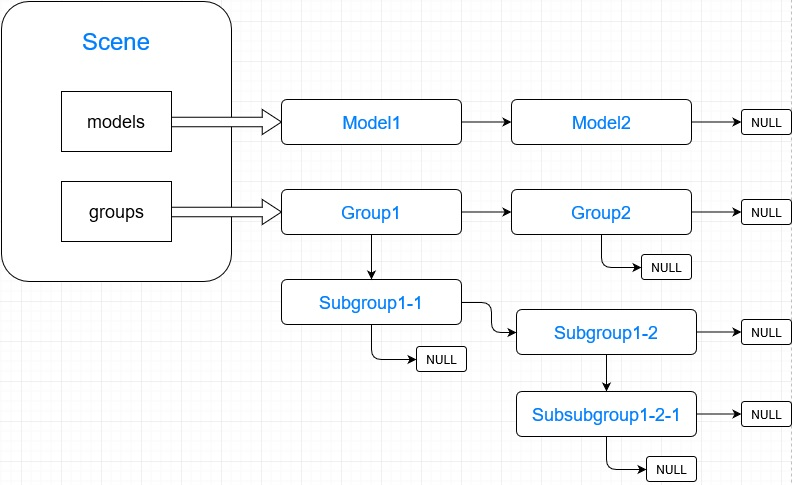
\includegraphics[scale=0.5]{imagens/structureComplete.jpg}
	\caption{Esquema representativo da estrutura de dados utilizada}
	\label{p1:fig:p1_estrutura}
\end{figure}


O modelo da estrutura de dados  \textit{sCommand} é implementado com tipo de comando, a informação e um apontador para o seguinte, como pode ser observado na figura \ref{p1:fig:p1_estruturacomando}:

\begin{figure}[htpb]
	\centering
	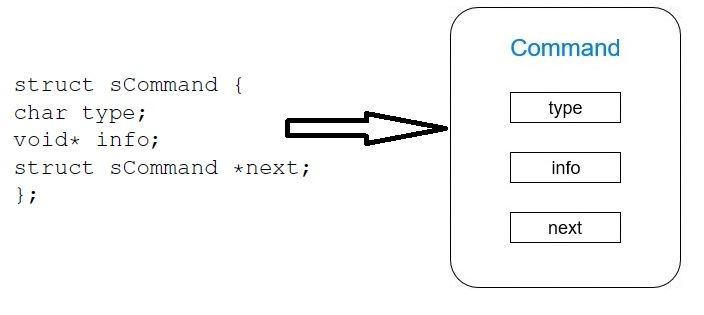
\includegraphics[scale=0.5]{imagens/structureCommand.jpg}
	\caption{Estrutura para Comando}
	\label{p1:fig:p1_estruturacomando}
\end{figure}

O modelo da estrutura de dados  \textit{sGroup} é implementado com uma lista de comandos referente a esse grupo e subgrupos, apontador para o subgrupo e um apontador para o seguinte, como pode ser observado na figura \ref{p1:fig:p1_estruturagroup}:

\begin{figure}[htpb]
	\centering
	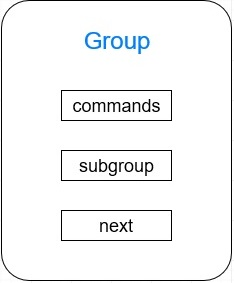
\includegraphics[scale=0.5]{imagens/structureGroup.jpg}
	\caption{Estrutura para Grupo}
	\label{p1:fig:p1_estruturagroup}
\end{figure}

O modelo da estrutura de dados  \textit{sModel} é implementado com um nome, número de pontos gerados, um conjunto de pontos e um apontador para o modelo seguinte, como pode ser observado na figura \ref{p1:fig:p1_estruturamodel}:

\begin{figure}[htpb]
	\centering
	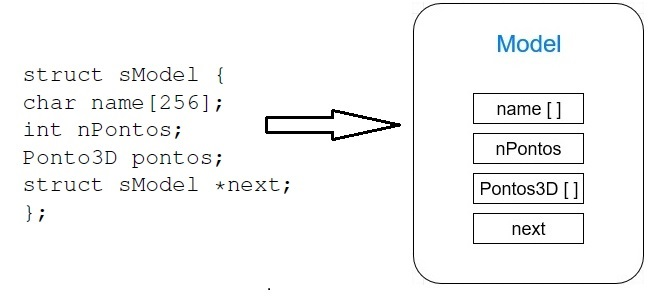
\includegraphics[scale=0.5]{imagens/structureModel.jpg}
	\caption{Estrutura para o Model}
	\label{p1:fig:p1_estruturamodel}
\end{figure}

\newpage
\section{ Descrição do ciclo de rendering}

Para a elaboração do rendering foi necessária a criação de funções que visam a conversão de símbolos gráficos num arquivo visual. 

A função \textit{drawGroup} é utilizada para arrancar o desenho dos grupos e respetivos subgrupos, mais uma vez de modo recursivo. 
\begin{Verbatim}
void drawGroup(struct sGroup* g, Scene s) {
     if(existe grupo) {
          glPushMatrix(); // guarda a matriz
          for(todos os comandos 'c' ){
                drawCommand(c, s);
           }
          drawGroup(subgrupo, s);
          drawGroup(grupo seguinte, s);
          glPopMatrix();// volta para a matriz guardada
    }
}
\end{Verbatim}


A função \textit{drawcommand} é utilizada para imprimir a lista de comandos referentes às transformações geométricas e impressão  dos modelos para o ecrã. 

\begin{Verbatim}
void drawCommand(struct sCommand* c, Scene s){
  if(tipo do comando == 'TRANSLAÇÃO' ){
     glTranslatef(dados do comando = 3 floats);
  }
  if(tipo do comando ==  'ROTAÇÃO'){
    glRotatef(Dados do comando = 4 floats);
  }
  if(tipo do comando == 'ESCALA'){
    glScalef(Dados do comando  = 3 floats);
  }
  if(tipo do comando == 'COR'){
    glColor3f(Dados do comando  = 3 floats);
  }
  if(tipo do comando == 'MODELAR'){
    drawModel(Dados do comando = nome do ficheiro, cena global );
  }
}

\end{Verbatim}


A função \textit{drawModel} é utilizada para desenhar os pontos correspondentes ao modelo em questão utiliza as funções \textit{add\_read\_Model} já explicadas anteriormente na secção do processo de leitura. 
\begin{Verbatim}
void drawModel(char* model, Scene s) {
   while(não for o modelo desejado){
      avança entre os modelos; 
   }
   if(não existir modelo){
      add_read_Model(model,&(s->models));// lê o modelo do ficheiro
      drawModel(model,s); //volta a tentar desenhar o modelo
   } else {
      glBegin(GL_TRIANGLES);
      for(todos os pontos ){
         glVertex3f(ponto);
      }
      glEnd();
   }
}
\end{Verbatim}


\chapter{Demo}

A Demo, para a segunda fase do projeto, corresponde ao modelo estático do Sistema Solar, e contem o Sol, os Planetas e Luas. Para a elaboração da Demo começou-se por criar o Sol que se encontra no centro do Sistema Solar, centrado nas coordenadas (0,0,0). Em seguida foram desenhados os planetas e respetivas luas pela sua  ordem.

Apesar de as distâncias entre os Planetas não estarem à escala, no que toca aos planetas tentou-se ser o mais fiel possivel, mas devido ao facto de o Sol ser imensamente maior que grande parte dos Planetas tivemos que fazer algumas alteraçõs às suas escalas, de modo a ser possível representar todos os Planetas e algumas das luas do Sistema Solar, não tendo planetas imensamente pequenos o que dificultaria a sua visualização. Esta decisão foi também tomada devido ao facto de que se seguíssemos as escalas reais à risca a Lua da Terra não seria desenhada por ser demasiado pequena.

\begin{figure}[htpb]
	\centering
	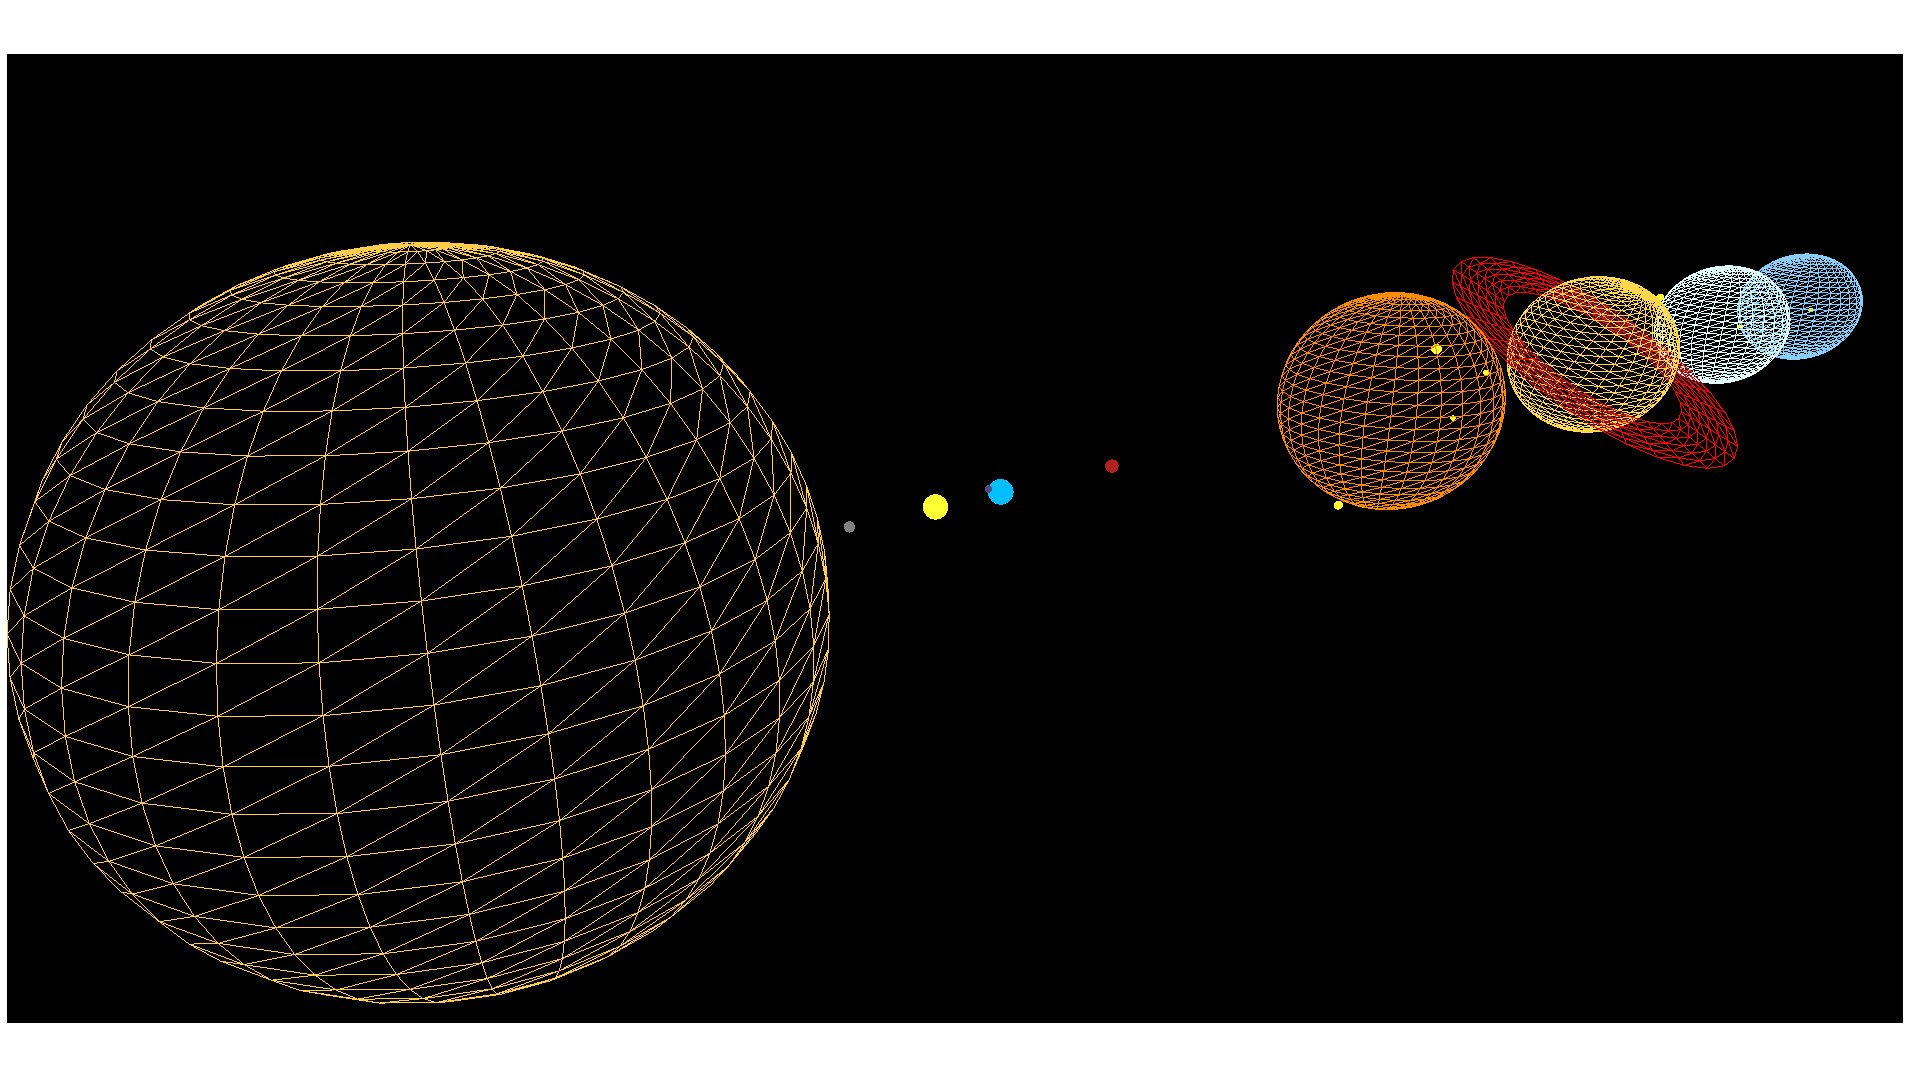
\includegraphics[scale=0.2445]{imagens/solarsystem.png}
	\caption{Sistema Solar com os planetas desenhados e Sol no centro}
	\label{p1:fig:p1_sistemasolar}
\end{figure}


Para desenhar Mercúrio e Vénus não existe grande diferença entre eles e o Sol, fazendo uma escala e uma translação colocamos estes planetas no sítio que desejamos com o tamanho mais indicado. Para os restantes planetas já temos que usar uma relação Pai-Filho, devido ao facto, de os restantes planetas a serem desenhados conterem uma ou mais Luas, ou, no caso de Saturno, um anel. Essa relação é feita no ficheiro XML colocando as luas ou aneis como filhos do Planeta a que pertencem. 




